
%% 
%% Copyright 2007, 2008, 2009 Elsevier Ltd
%% 
%% This file is part of the 'Elsarticle Bundle'.
%% ---------------------------------------------
%% 
%% It may be distributed under the conditions of the LaTeX Project Public
%% License, either version 1.2 of this license or (at your option) any
%% later version.  The latest version of this license is in
%%    http://www.latex-project.org/lppl.txt
%% and version 1.2 or later is part of all distributions of LaTeX
%% version 1999/12/01 or later.
%% 
%% The list of all files belonging to the 'Elsarticle Bundle' is
%% given in the file `manifest.txt'.
%% 
%% Template article for Elsevier's document class `elsarticle'
%% with harvard style bibliographic references
%% SP 2008/03/01

\documentclass[preprint,9pt]{elsarticle}

%% Use the option review to obtain double line spacing
%% \documentclass[authoryear,preprint,review,12pt]{elsarticle}

%% Use the options 1p,twocolumn; 3p; 3p,twocolumn; 5p; or 5p,twocolumn
%% for a journal layout:
%% \documentclass[final,1p,times,authoryear]{elsarticle}
%% \documentclass[final,1p,times,twocolumn,authoryear]{elsarticle}
%% \documentclass[final,3p,times,authoryear]{elsarticle}
%% \documentclass[final,3p,times,twocolumn,authoryear]{elsarticle}
%% \documentclass[final,5p,times,authoryear]{elsarticle}
%% \documentclass[final,5p,times,twocolumn,authoryear]{elsarticle}

%% For including figures, graphicx.sty has been loaded in
%% elsarticle.cls. If you prefer to use the old commands
%% please give \usepackage{epsfig}

%% The amssymb package provides various useful mathematical symbols
\usepackage{amsmath,amssymb,bm}
%\usepackage[dvips,colorlinks=true,citecolor=green]{hyperref}
\usepackage[colorlinks=true,citecolor=green]{hyperref}
%% my added packages
\usepackage{verbatim}
\usepackage{caption}
\usepackage{subcaption}
\usepackage{booktabs} % for nice tables
\usepackage{csvsimple} % for csv read
\usepackage{graphicx}
%\usepackage[outdir=//odroid-sensors/sensors/aidd/reports/journal_papers/MSSP_Paper/Figures/]{epstopdf}
%\usepackage{breqn}
\usepackage{multirow}
% matrix command 
\newcommand{\matr}[1]{\mathbf{#1}} % bold upright (Elsevier, Springer)
% vector command 
\newcommand{\vect}[1]{\mathbf{#1}} % bold upright (Elsevier, Springer)
\newcommand{\ud}{\mathrm{d}}
\renewcommand{\vec}[1]{\mathbf{#1}}
\newcommand{\veca}[2]{\mathbf{#1}{#2}}
\renewcommand{\bm}[1]{\mathbf{#1}}
\newcommand{\bs}[1]{\boldsymbol{#1}}
\graphicspath{{Figures/}{//odroid-sensors/sensors/aidd/reports/journal_papers/MSSP_Paper/Figures/}}
%\graphicspath{ {Graphics/Figures/} }
%% The amsthm package provides extended theorem environments
%% \usepackage{amsthm}
%% The lineno packages adds line numbers. Start line numbering with
%% \begin{linenumbers}, end it with \end{linenumbers}. Or switch it on
%% for the whole article with \linenumbers.
%% \usepackage{lineno}
\journal{Mechanical Systems and Signal Processing}

\begin{document}
	\begin{frontmatter}
		\addcontentsline{toc}{section}{References}
		%% Title, authors and addresses
		%% use the tnoteref command within \title for footnotes;
		%% use the tnotetext command for theassociated footnote;
		%% use the fnref command within \author or \address for footnotes;
		%% use the fntext command for theassociated footnote;
		%% use the corref command within \author for corresponding author footnotes;
		%% use the cortext command for theassociated footnote;
		%% use the ead command for the email address,
		%% and the form \ead[url] for the home page:
		%% \title{Title\tnoteref{label1}}
		%% \tnotetext[label1]{}
		%% \author{Name\corref{cor1}\fnref{label2}}
		%% \ead{email address}
		%% \ead[url]{home page}
		%% \fntext[label2]{}
		%% \cortext[cor1]{}
		%% \address{Address\fnref{label3}}
		%% \fntext[label3]{}
		
		\title{Full Wavefield Processing by Using FCN for Delamination Detection}
		
		%% use optional labels to link authors explicitly to addresses:
		%% \author[label1,label2]{}
		\address[IFFM]{Institute of Fluid Flow Machinery, Polish Academy of Sciences, Poland}
		
		\author{Abdalraheem A. Ijjeh\fnref{IFFM}}
		\author{Saeed Ullah \fnref{IFFM}}
		\author{Pawel Kudela\corref{cor1}\fnref{IFFM}}
		\ead{pk@imp.gda.pl}
		%\ead{pfiborek@imp.gda.pl}
		%\author{Tomasz Wandowski \fnref{IFFM}}	
		
		\cortext[cor1]{Corresponding author}
		
		\begin{abstract}
		
		\end{abstract}
		
		\begin{keyword}
			%% keywords here, in the form: keyword \sep keyword
			Lamb waves \sep dispersion curves \sep structural heath monitoring \sep damage detection \sep deep learning \sep Convolutional neural networks. \sep fully convolutional neural network
			%% PACS codes here, in the form: \PACS code \sep code
			
			%% MSC codes here, in the form: \MSC code \sep code
			%% or \MSC[2008] code \sep code (2000 is the default)
			
		\end{keyword}
		
	\end{frontmatter}
	%% main text
	%%%%%%%%%%%%%%%%%%%%%%%%%%%%%%%%%%%%%%%%%%%%%%%%%%

	\section{Introduction}
	%%%%%%%%%%%%%%%%%%%%%%%%%%%%%%%%%%%%%%%%%%%%%%%%%%
	Composite materials have a wide range of applications in various industries, due to their characteristics such as high strength, low density, resistance to fatigue, and corrosion.  
	However, damage can occur in composites materials due to impacts resulting from the lack of reinforcement in the out-of-plane direction.
	In particular, laminated composite materials are more sensitive to delamination damage due to weak transverse tensile and interlaminar shear strengths.
	Delamination can alter the compression strength of composite laminate, and gradually affect the composite to encounter failure by buckling. 
	Delaminations can seriously decrease the performance of composites structures, accordingly, delamination detection in its early stages can significantly help to avoid catastrophic structural collapses.
	
	One of the conventional techniques for damage identification for nondestructive evaluation (NDE) involves arrays of transducers that can be mounted or embedded in the structures for registering the response of the guided wave propagation.
	However, damage identification regarding structures with curved and deformable geometry can be inaccurate when using transducers array, also, damage influence maps resulted from transducer array have low resolution, due to the small number of sensing points. 
    Accordingly, this issue of low resolution damage influence map can be solved by utilising a Scanning Laser Doppler Vibrometry (SLDV), which is a non-contact technique dedicated to full wavefield measuring vibration and guided wave propagation by registering measurements for a dense mesh of measuring points spanned over the area of the investigated structure.
    Consequently, SLDV produces a full wavefield of measurements with high resolution of damage influence maps which can significantly improve the process of damage detection and localization. 
    
    Conventional damage detection and localization methods focus on patterns extraction from registered measurements (whether from transducers array or SLDV) and accordingly make decisions based on the patterns ~\cite{Gul2009}. 
    Moreover, conventional methods for patterns recognition requires feature selection and classification (handcrafted features). 
	These conventional methods can perform efficient damage detection, however, these methods depend on selected features from their scope of measurement, accordingly, introducing new patterns will cause them to fail in detecting the damage.
	Moreover, these methods could fail in detecting damage when dealing with big data requiring a complex computation of damage features.
    
    

    In this work, we investigate delamination since it is one of the most dangerous damage types.

\subsection{Review of Damage detection Techniques within composite materials }	
Different approaches were applied for detecting damage in composite materials. Yet, A well-known method that is used for that purpose are the Lamb wave techniques. In general, we can define Lamb waves as an elastic vibration that can propagate in solid structures (plates wrapped into cylindrical pipes or vessels or plates cut into thin strips, etc.) with free boundaries. In which, Lamb waves consist of two types of waves, symmetric ($S0,S1,S2...$) and anti-symmetric ($A0,A1,A2...$) modes , and each mode can propagate independently of the other. Lamb waves ($A0$ mode) are commonly used due to the fact that it can propagate for long distances with little dispersion, and no higher modes are present to turbulence the resulting response wave~\cite{Valed2000}.
	
The earliest application of Lamb waves on composite materials was performed by Saravanos~\cite{doi:10.2514/6.1994-1754}, in which he explored the possibility of detecting delamination in composite beams using Lamb waves. Later, Percival and Birt~\cite{Percival1997}, who started focusing their work on the two fundamental Lamb wave modes have concluded the same. Damage Detection in composite materials of other forms was also inspected by Seale~\cite{Seale1998}, who examined fatigue and thermal damage. Also, Tang~\cite{Tang1989} examined the sensitivity of Lamb wave propagation to fiber fracture.

There are plenty of methods which utilizes Lamb waves for damage detection in SHM. One of the successful approaches has been done by two separate groups (Cawley and Soutis) at Imperical College, Cawley's group has developed polyvinylidenefluride(PVDS) transducers in which it can generate Lamb waves and receive it, those generated waves are highly focused. Soltis's group main focus was on sensor placement and signal processing issues~\cite{Valed2000,Valed2000a,Valed2001}. They have chosen to use Lead–Zirconate–Titanate (PZT) actuators and sensors over PVDF since they require a factor of ten less voltage to generate Lamb waves. Moreover, implemented Lamb wave techniques in SHM are broadly reported to be beneficial, efficient and sensitive in detecting defects in metallic structures, disbonds and delaminations in composite structures~\cite{Boller2000,Diamanti2004,Su2006,Raghavan2007,Diamanti2007} \newline Authors in~\cite{Ng2009} 
	

In this work, we went a step further, we used a large collection of signals (animation of propagating elastic waves), which are registered on very dense grid of points resembles scanning laser vibrometer measurements. Such collection of signals is often called full wave-field. 
It was found
%%%%%%%%%%%%%%%%%%%%%%%%%%%%%%%%%%%%%%%%%%%%%%%%%%%%%
\section{Methodology}
%%%%%%%%%%%%%%%%%%%%%%%%%%%%%%%%%%%%%%%%%%%%%%%%%%%%%
%%%%%%%%%%%%%%%%%%%%%%%%%%%%%%%%%%%%%%%%%%%%%%%%%%%%%
\subsection{Dataset}
%%%%%%%%%%%%%%%%%%%%%%%%%%%%%%%%%%%%%%%%%%%%%%%%%%%%%
In this work, we have generated a large dataset of 475 cases of a full wavefield of propagating Lamb waves in a plate made of carbon fibre-reinforced plastic (CFRP).
The time domain spectral element method was used for simulation of Lamb wave interaction with delamination.
For each case single delamination was modelled by using the method of splitting nodes between appropriate spectral elements. 
It was assumed that the composite laminate is made of eight layers of total thickness 3.9 mm.
The delamination was modelled between the third and fourth layer (see Fig.~\ref{fig:plate_setup} for details).
It should be noted that the figure shows exaggerated cross-section through the delamination. 
Zero-volume delamination was assumed in the model. 
For each case delamination location was selected randomly so that interaction of guided waves excited at the plate centre with delamination is different for each case.
It includes cases when delamination is located at the edge of the plate which is the most difficult to identify by signal processing methods.
Additionally, the size of the delamination was randomly simulated by selecting ellipse minor and major axis from the interval 5--20 mm.
Also the angle between delamination major axis and horizontal axis was randomly selected.
\begin{figure}
	\centering
	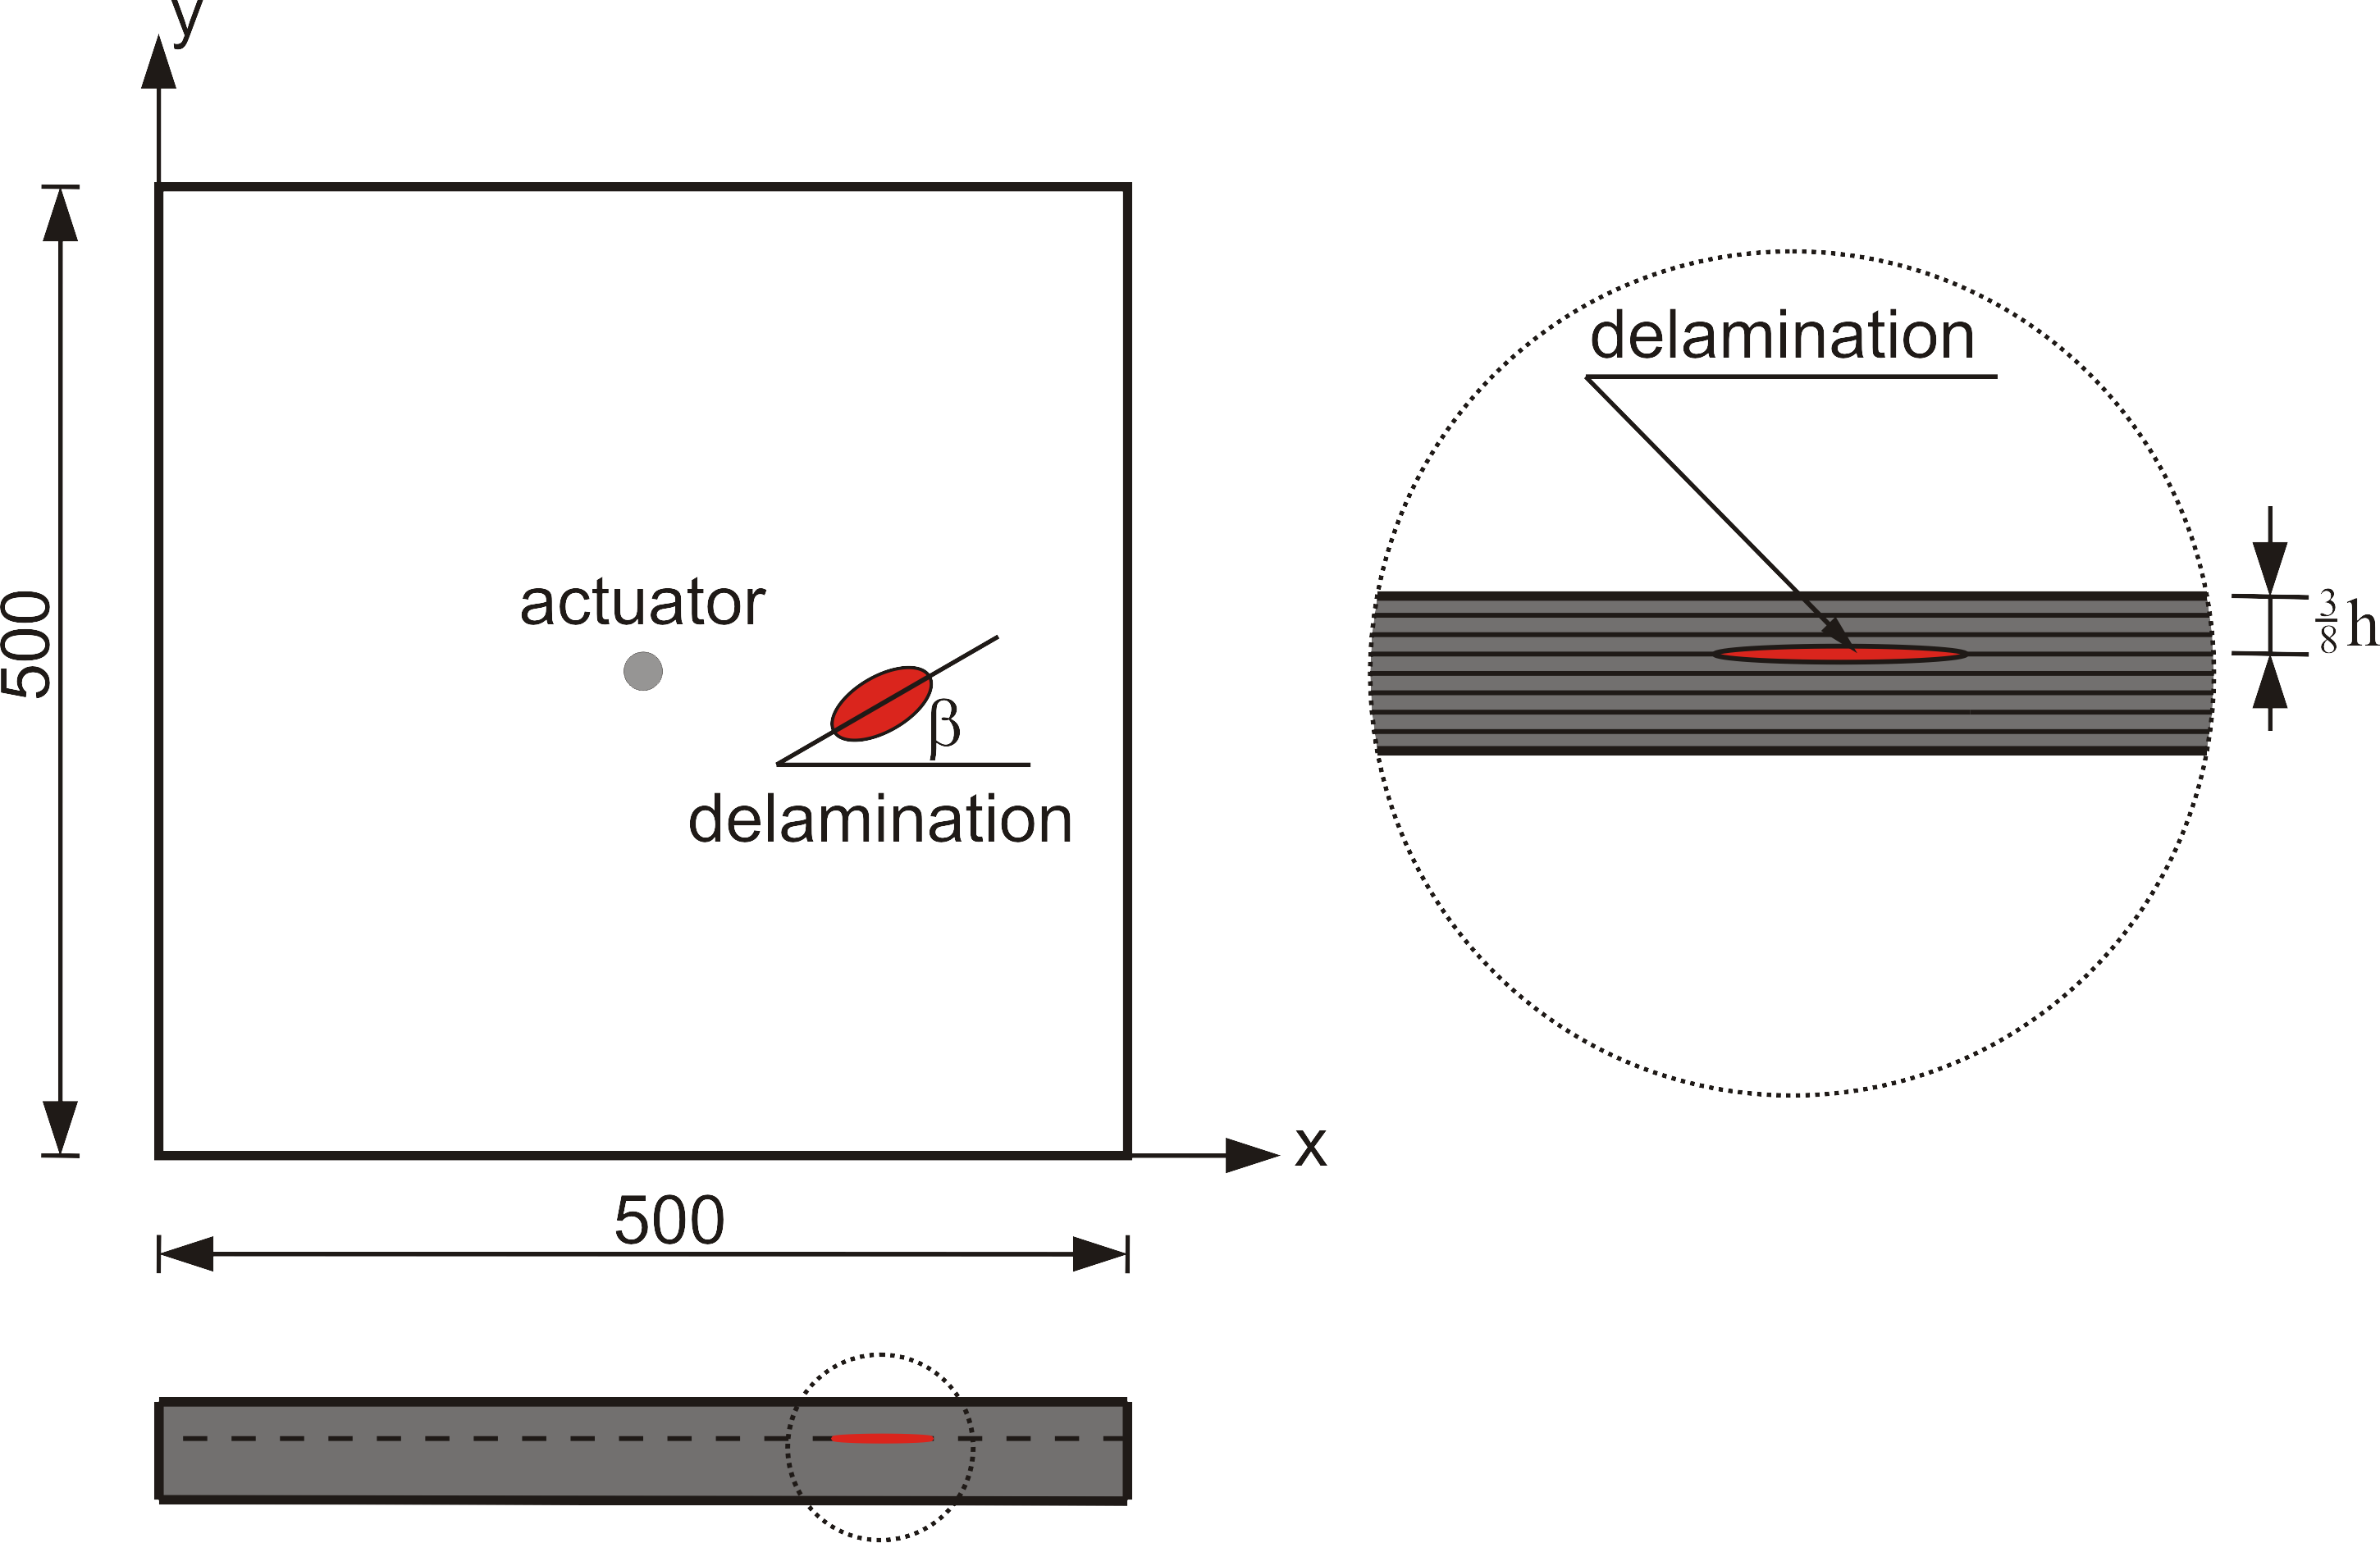
\includegraphics[scale=0.8]{plate_delam_arrangement_MSSP.png}
	\caption{Setup for computing Lamb wave interactions with delamination.}
	\label{fig:plate_setup}
\end{figure}

The output from the top and bottom surface of the plate in the form of particle velocities at the nodes of spectral elements were projected on the uniform grid of 500\(\times\)500 points by using shape functions of elements (see Parallel spectral element method for guided wave based structural health monitoring paper for detail).
It essentially resembles measurements acquired by scanning laser Doppler vibrometer (SLDV) in the transverse direction (perpendicular to the plate surface).

%%%%%%%%%%%%%%%%%%%%%%%%%%%%%%%%%%%%%%%%%%%%%%%%%%%%
\subsection{Signal processing strategy}
%%%%%%%%%%%%%%%%%%%%%%%%%%%%%%%%%%%%%%%%%%%%%%%%%%%%
\begin{figure}
	\centering
	\includegraphics[scale=0.8]{FCN_adaptive_filtering_diagram_MSSP.png}
	\caption{Diagram of signal processing strategy by the proposed Fully Convolutional Network (left branch) in comparison to signal processing utilising adaptive wavenumber filtering method (right branch). }
	\label{fig:sig_proc_strategy}
\end{figure}

%%%%%%%%%%%%%%%%%%%%%%%%%%%%%%%%%%%%%%%%%%%%%%%%%%%%	
\subsection{Adaptive wavenumber filtering}
%%%%%%%%%%%%%%%%%%%%%%%%%%%%%%%%%%%%%%%%%%%%%%%%%%%%%

%%%%%%%%%%%%%%%%%%%%%%%%%%%%%%%%%%%%%%%%%%%%%%%%%%%%%
\subsection{Fully Convolutional Network approach}
%%%%%%%%%%%%%%%%%%%%%%%%%%%%%%%%%%%%%%%%%%%%%%%%%%%%%
In this work, A deep learning approach for delamination detection in composite materials is presented. 
%%%%%%%%%%%%%%%%%%%%%%%%%%%%%%%%%%%%%%%%%%%%%%%%%%%%%
\subsubsection{Data preprocessing}
%%%%%%%%%%%%%%%%%%%%%%%%%%%%%%%%%%%%%%%%%%%%%%%%%%%%%
It should be noted that the output from the wave propagation model is in the form of 3D matrix which contains amplitudes of propagating waves at location \((x, y)\) and time \(t\). We can look at it as a set of frames of propagating waves at discrete time moments \(t_k\).

The data preprocessing as it is indicated in Fig. ?? include a step of computation of root mean square value:
\begin{equation}
\hat{s}(x,y) = \sqrt{\frac{1}{N}\sum_{k=1}^{N} s(x,y,t_k)^2}
\end{equation}
where number of sampling points \(N\) was 512.
In this way, dataset was collapsed to 475 2D matrices in which amplitudes are stored as double precision values.
The next step was conversion of these matrices to greyscale images (colour image quantisation).
Colour scale values of obtained images vary between (\(0 - 255\)) hence normalization
to a range of (\(0-1\)) was applied to enhance the optimizer function during the learning process. 
Furthermore data augmentation was achieved by flipping images vertically, horizontally and diagonally to enhance the learning process through enabling the model to learn and recognize new complex patterns.
%%%%%%%%%%%%%%%%%%%%%%%%%%%%%%%%%%%%%%%%%%%%%%%%%%%%%
\subsubsection{Basic concept of Fully Convolutional Network}
%%%%%%%%%%%%%%%%%%%%%%%%%%%%%%%%%%%%%%%%%%%%%%%%%%%%%
The main purpose of such approach is to automatically perform feature extraction by training a model using full wavefield images, hence, it will learn by itself to recognise the patterns and detect the delamination and localize it.
In our work we are using fully convolutional network (FCN), which aims to perform pixel-wise segmentation by classifying every pixel of the input image as damaged or not. 
Therefore, several models were implemented for that purpose.

The idea behind FCN is to stack a group of convolutional layers in an encoder-decoder style. 
The encoder is capable for downsampling the input image through convolutions with strides, consequently, resulting in a compressed feature representation of the input image, and the decoder is capable to upsample the image with compressed features applying techniques like transposed convolution with strides and upsampling with interpolation (e.g. bilinear or nearest).


In order to reduce overfitting in the models, some techniques were applied such as adding dropouts to layers.

For the output layer, we have applied two activation functions in separate experiments, the first one is softmax and the second one is sigmoid. 
The softmax function calculates the probability of the damaged and the undamaged for every single pixel, hence, the summation of the two probabilities must equal one. Eqn.~\ref{softmax} illustrates the softmax, where \(P(x)_{i}\) is the probability of each target class \(x_{j}\) over all possible target classes \(x_{j}\), C in our case are two classes  (damaged and undamaged.
To predict the output label of the detection (\(y_{pred}\)) which represent the probability of damaged and undamaged we applied the \(argmax\) function to select the maximum probability of the softmax activation function.
\begin{equation}
P(x)_{i} = \frac{e^{x_{i}}}{\sum_{j}^{C} e^{x_{j}}}
\label{softmax}
\end{equation} 
\begin{equation}
y_{pred} = aragmax_{i}\left( \left[P(x)_{i}\right]\right)
\label{argmax}
\end{equation}

When using sigmoid in the output layer, it produces a vector of values between (\(0\) and \(1\)) indicating the damage weight for each pixel. 
Low values indicate low damage probability and high output values indicate high damage probability. Eqn.~\ref{sigmoid} illustrates the sigmoid function, 
where \(z\) is the summation of adjustable weights \(\{w_0,w_1,...,w_n \}\) multiplied by input variables (from previous layer) \(\{x_0,x_1,_...,x_n\}\) and a bias \(b\) as shown in Eqn~\ref{z}.
\begin{equation}
	\sigma(z) = \frac{1}{1+e^{-z}}
	\label{sigmoid}
\end{equation}
\begin{equation}
	z= \sum_{i=0}^{n}  w_i\times x_i +b
	\label{z}
\end{equation}
Selecting the loss function is a crucial task in deep learning since it measures how good the model predicts.
We have applied two types of losses based on the used function in the final activation layer: Binary cross-entropy (BCE) loss function applied with a sigmoid activation function in the output layer, Categorical cross-entropy (CCE) loss function with a softmax activation in the output layer which is also called softmax loss function.
Eqn.~\ref{BCE} illustrates the BCE, where \(\hat{Y}\) represents the predicted vector values and \(Y\) represents the ground truth vector values, when \(\hat{Y} \approx Y\) then the BCE will be almost \(0\) meaning that the model was able to predict the output, so, the aim is to reduce the loss function to the minimum value.
\begin{equation}
	BCE = (1-Y)log(1-\hat{Y})+Ylog(\hat{Y})
	\label{BCE}
\end{equation}
Eqn.~\ref{CCE} illustrates the CCE, where \( P(x)_{i}\) is the softmax value of the target class. 
\begin{equation}
CCE = -log\left( P(x)_{i} \right)
\label{CCE}
\end{equation}

Moreover, we have applied intersection over union (IoU) as our accuracy metric. 
IoU is applied to find the intersection area between the ground truth value and the predicted value eqn.~\ref{IoU} illustrates the IoU metric.
The intersection between the predicted and the ground truth values is simply calculated through multiplying their values then summing the resulted values.
As we mentioned earlier the ground truth values are either \((0\) or \(1)\) thus only the predicted values larger than \(0\) and their ground truth label is \(1\) will be counted, the rest values will equal to \(0\). 
The union can be calculated by summing all values in both the predicted and the ground truth  vectors, then we subtract the intersection from their sum.
Our main goal is to maximize the IoU accuracy metric, since the higher the IoU, the higher the accuracy of the predicted delamination damage.
\begin{equation}
IoU = \frac{Intersection}{Union} = \frac{\hat{Y} \cap Y}{\hat{Y} \cup Y} 
\label{IoU}
\end{equation}

Furthermore, during training the model our focus is to minimize the loss and maximize the accuracy metric by converting it into an optimization problem. 
The optimizer is responsible for updating the model learnable parameters such as filters weights and biases in a way the overall loss is minimized and the accuracy is maximized.
In our work, Adam optimizer was applied, which is considered as a combination of RMSprob and Stochastic Gradient Descent (SGD)~\cite{Kingma2015}. 

In the next subsections we are going to present three FCN models for pixel wise semantic segmentation in order to detect and localize delaminations.
%%%%%%%%%%%%%%%%%%%%%%%%%%%%%%%%%%%%%%%%%%%%%%%%%%%%%
\subsubsection{U-net based model}
%%%%%%%%%%%%%%%%%%%%%%%%%%%%%%%%%%%%%%%%%%%%%%%%%%%%%
Our first FCN model is the U-net model, which was introduced by Ronneberger et al.~\cite{Ronneberger2015} for biomedical image segmentation constructed from two parts encoder and decoder. 
This architecture consists of three sections: The downsampling section, The bottleneck, and the upsampling section. 
The downsampling section holds several contraction blocks. 
Each block takes an input applies two (\(3\times3\)) convolution layers followed by a (\(2\times2\)) max pooling with a (\(2\times2\)) strides. 
The number of convolutional filters is doubled after each downsampling block so that architecture can learn the complex patterns effectively. 
The bottleneck layer meddles between the downsampling section and the upsampling section. 
It composed of two (\(3\times3\)) convolution layers followed by (\(2\times2\)) up convolution layer (Transpose convolution).
The upsampling section is similar to downsampling section, it also consists of several upsampling blocks. 
Each block passes the input to two (\(3\times3\)) convolution layers followed by a (\(2\times2\)) Convolutional transposed layer (upsampling). 
Moreover, after each block, the number of feature maps used by convolutional layer get half to keep the model symmetrical. 
Further, skip connections were added by appending feature maps of the downsampling block with the corresponding upsampling block to retrieve lost spatial information during the downsampling to due to decreasing the input resolution.
By doing so, the model ensures that the feature maps which were learned during the image downsampling will be utilised to reconstruct it. 
Furthermore, to enhance the model training performance we applied a technique called batch-normalization (BN)~\cite{Ioffe2015}.
The term "batch" was added because, during training, we normalize the output of the previous layer for each batch, applying a transformation that keeps the mean activation value close to \(0\) and the activation standard deviation close to \(1\), which eventually enhances the learning rate.
\begin{figure} [h!]
	\begin{center}
		\includegraphics[scale= 0.8]{Unet_model.png}
	\end{center}
	\caption{U-Net architecture.} 
	\label{fig:Unet}
\end{figure}
Fig.~\ref{fig:Unet} presents the model architecture showing the path of the input of a full wavefield image of a size (\(512\times512\)) through the downsampling, bottleneck then the upsampling finally to the output which contains the prediction of delamination size and location. 
In the downsampling section,
Each layer performs (\(3\times3\)) convolution, followed by Relu activation function followed by BN operation.
Further, the Transmission Down layer contains a Maxpool function with (\(2\times2\)) pooling filter and a (\(2\times2\)) strides that picks the maximum value in a local pool filter in one feature map (or \(n\)-feature maps), resulting in a reduction in the dimension of feature maps~\cite{Lecun2015}, consequently, reducing computation complexity.
The bottleneck section is the deepest section in the model, it contains two convolutional layers, with 256 filters which helps the model to learn and recognize new complex patterns.
The Upsampling section is similar to the down sampling section, in which each layer  performs (\(3\times3\)) convolution, followed by Relu activation function followed by BN operation. But, for the Transmission Up layer it perform the opposite of downsampling.
The purpose is to retrieve the dimensions before sampling and increase the resolution of the images. 
For this model we have applied a (\(3\times3\))Transposed convolution with (\(2\times2\)) strides.
Transposed convolution layer differs from the regular upsampling function, by introducing learnable parameters regarding the transposed convolution filters that enhance the learning process of the model, therefore, new patterns are recognized. 


\subsubsection{FCN-DenseNet based model}
FCN-DenseNet was introduced by Simon Jegou et al.~\cite{Jegou} for semantic segmentation, it was originally based on the DenseNet model proposed by Gao Huang et al.~\cite{Huang}. 
The main advantage of FCN-DenseNet over DenseNet is the extra utilising of feature maps by adding the upsampling path to the model.
FCN-DenseNet is composed of downsampling path, upsampling path and skip connection.
Skip connections from the downsampling path to the corresponding upsampling path are essential for recovering spatially detailed information by reusing feature maps.
 
The essential component in FCN-DenseNet is the dense block.
The purpose of the dense block is to concatenate layer input (feature maps) with its output (feature maps) to emphasize spatial details information.
A dense block is constructed from \(n\) varying number of layers, each layer is composed of a series of operations.
Figure~\ref{dense_block} presents the architecture of dense block has an input (\(x\)) (input image or output of transition layer) with \(k\) feature maps is concatenated with the output of first layer and this process is recursively performed for all layers in the dense block ending up with output (\(y\)) with a (\(n\times k\)) feature maps. 
Transition down layer was introduced to reduce the spatial dimensionality of the feature maps, to perform that a (\(1\times 1\))  convolution followed by (\(2\times2\)) Maxpool operation are applied. 

\begin{figure} [h!]
	\begin{center}
		\includegraphics{DenseBlock_layer.png}
	\end{center}
	\caption{Dense Block architecture.} 
	\label{dense_block}
\end{figure}

For the transition up layer, it was introduced in FCN-DenseNet to recover the input spatial resolution, to do that a transpose convolution operation is performed which upsamples the previous feature maps.
Feature maps emerging from upsampling are concatenated with the ones resulting from the skip connection forming the input to a new dense block.
During the upsampling, the input to the dense block is not concatenated with its output to overcome the overhead of memory shortage since the upsampling path expands the spatial resolution of the feature maps.
Table~\ref{layers} presents the architecture of a single layer, the transition down  and transition up layers in details.

\begin{table}[]
	\centering
	\scriptsize
	\begin{tabular}{|c|l|c|l|c|}
		\cline{1-1} \cline{3-3} \cline{5-5}
		\textbf{Layer} &  & \textbf{Transition Down} &  & \textbf{Transition Up} \\ \cline{1-1} \cline{3-3} \cline{5-5} 
		Batch Normalization &  & Batch Normalization &  & \multirow{5}{*}{\begin{tabular}[c]{@{}c@{}}(\(3\times3\)) Transposed Convolution, \\ strides = (\(2\times2\))\end{tabular}} \\ \cline{1-1} \cline{3-3}
		Relu &  & Relu &  &  \\ \cline{1-1} \cline{3-3}
		(\(3\times3\)) Convolution &  & (\(1\times1\)) Convolution &  &  \\ \cline{1-1} \cline{3-3}
		\multirow{2}{*}{Dropout \(p = 0.2\)} &  & Dropout \(p = 0.2\) &  &  \\ \cline{3-3}
		&  & (\(2\times2\)) Maxpooling &  &  \\ \cline{1-1} \cline{3-3} \cline{5-5} 
	\end{tabular}
	\caption{Layer, Transition Down and Transition Up layers.} 
	\label{layers}
\end{table}

Our constructed model is composed of \(3\) dense blocks in the downsampling path, one dense block in bottleneck and 3 dense blocks for the upsampling path. 
Each dense block in the downsampling and upsampling paths consists of \(2\) layers, the bottleneck dense block consists of \(4\) layers.
The model input is a full wavefield image with size of (\(512\times 512\)), at the beginning , we perform a  convolution operation and concatenate the original input with the output then the concatenated output is fed into the first dense block that consist of (\(2\)) layers, each layer is composed of BN followed by Relu then (\(3\times3\)) convolution with same padding is applied followed by a dropout with probability \(p = 0.2\).
Then, the output of the first dense layer is concatenated with its input are fed into a transition down layer composed of BN followed by Relu then (\(1\times1\)) convolution followed by a dropout with probability \(p = 0.2\) then (\(2\times2\)) Maxpool with strides of (\(2\times2\))  , this process is repeated till the bottleneck dense block.
The bottleneck dense block consist of 4 layers
The output of the bottleneck is directed into upsampling path starting with transition up layer.
Accordingly, the output of the transition up layer is concatenated with the corresponding dense block output in the downsampling path, the final layer in the network is  (\(1\times1\)) convolution followed by a sigmoid function to calculate the probability of damage for each pixel.
\begin{figure} [h!]
	\begin{center}
		\includegraphics[scale= 0.8]{FCN_dense_net.png}
	\end{center}
	\caption{FCN-DenseNet architecture.} 
	\label{fcn}
\end{figure}
Figure~\ref{fcn} illustrates the FCN-DenseNet architecture for image segmentation used for delamination detection.



\subsubsection{FCN-VGG16}
In this model we address the use of VGG16-based encoder~\cite{Simonyan2015} with 13-convolutional layers.
VGG16 encoder is composed of convolutional layers, pooling layers and dense layers, and it was used for classification purposes. 
In our last model, we employed an encoder decoder scheme for pixel wise image segmentation. 
Both encoder and decoder layers were trained from scratch.
Figure~\ref{vgg16} presents the architecture of VGG16- encoder decoder model. 
The model consists of two paths: downsampling and upsampling.
The downsampling path consists of \(5\) convolutional blocks,  with a total \(13\) convolutional layers  with same padding and kernel size (\(3\times3\))and 32 filters for each layer, followed by BN and activation function Relu.
Each convolutional layer is responsible for extracting high level features from the input image such as edges.
A Maxpool operation with pool size of (\(2\times2\))  and (\(2\times2\)) strides followed by dropout is performed after each convolutional block. 
The upsampling path is introduced to recover spatial resolution, it also has \(5\) convolutional blocks with a total \(13\) convolutional layers  with same padding and kernel size (\(3\times3\))and 32 filters for each layer, followed by BN and activation function Relu.
For upsampling, bilinear interpolation with (\(2\times2\)) kernel size is applied.
Skip connections were added between downsampling blocks and the corresponding upsampling blocks in order to enhance recovering fine-grained details by enabling feature reusability from earlier layers.
\begin{figure} [h!]
	\begin{center}
		\includegraphics[scale=0.8]{VGG16_encoder_decoder.png}
	\end{center}
	\caption{VGG16 encoder decoder architecture.} 
	\label{vgg16}
\end{figure}


\section{Results and Discussions}

%%%%%%%%%%%%%%%%%%%%%%%%%%%%%%%%%%%%%%%%%%%%%%%%%%
\section{Conclusions}
	
	%%%%%%%%%%%%%%%%%%%%%%%%%%%%%%%%%%%%%%%%%%%%%%%%%%

	%\appendix


\section*{}

	
\section*{ }
\bibliography{report}{}
\bibliographystyle{num_order}
	
	
\end{document}


